\chapter{Separating Hyperplanes, Lagrange Multipliers, and Convex Duality}
% \documentclass[draft,11pt]{article}
%\documentclass[11pt]{article}
%%  RASMUS  packages
\usepackage{blindtext}
\usepackage[usenames,dvipsnames,svgnames,table]{xcolor}
\usepackage{enumitem}
\usepackage{caption}
\usepackage{placeins}
\usepackage{graphicx}

\usepackage{fancybox}
\usepackage{hyperref}

\usepackage{amsmath,amsfonts,amsthm,amssymb,xcolor}
% \let\amsboldsymbol\boldsymbol % if you want to see the bad
% boldsymbol for comparison
\usepackage{bm} % fixes boldsymbol

\usepackage{nicefrac}

\usepackage{float}


% switched to algorithm2e in lecture 9
% \usepackage{algorithm} %ctan.org\pkg\algorithms
% \usepackage{algorithmic}
% \usepackage{algorithmicx}
% \usepackage[noend]{algpseudocode}

\newtheorem{theorem}{Theorem}[section]
\newtheorem{corollary}[theorem]{Corollary}
\newtheorem{lemma}[theorem]{Lemma}
\newtheorem{observation}[theorem]{Observation}
\newtheorem{proposition}[theorem]{Proposition}
\newtheorem{claim}[theorem]{Claim}
\newtheorem{fact}[theorem]{Fact}
\newtheorem{assumption}[theorem]{Assumption}
\newtheorem{warning}[theorem]{Warning}
\newtheorem{conjecture}[theorem]{Conjecture}

\theoremstyle{definition}
\newtheorem{definition}[theorem]{Definition}
\newtheorem{remark}[theorem]{Remark}

\newtheorem*{theorem*}{Theorem}
\newtheorem*{corollary*}{Corollary}
\newtheorem*{conjecture*}{Conjecture}
\newtheorem*{lemma*}{Lemma}
\newtheorem*{thm*}{Theorem}
\newtheorem*{prop*}{Proposition}
\newtheorem*{obs*}{Observation}
\newtheorem*{definition*}{Definition}
\newtheorem*{example}{Example}
\newtheorem*{remark*}{Remark}
\newtheorem*{rec*}{Recommendation}

\newenvironment{fminipage}%
  {\begin{Sbox}\begin{minipage}}%
  {\end{minipage}\end{Sbox}\fbox{\TheSbox}}

\newenvironment{algbox}[0]{\vskip 0.2in
\noindent 
\begin{fminipage}{6.3in}
}{
\end{fminipage}
\vskip 0.2in
}


\let\muchl\ll

\def\pleq{\preccurlyeq}
\def\pgeq{\succcurlyeq}
\def\pge{\succ}
\def\ple{\prec}

\def\Approx#1{\approx_{#1}}

%\def\Span#1{\textbf{Span}\left(#1  \right)}
\def\bvec#1{{\mbox{\boldmath $#1$}}}




\def\prob#1#2{\mbox{Pr}_{#1}\left[ #2 \right]}
\def\pvec#1#2{\vec{\mbox{P}}^{#1}\left[ #2 \right]}
\def\expec#1#2{{\mathbb{E}}_{#1}\left[ #2 \right]}
\def\var#1{\mbox{\bf Var}\left[ #1 \right]}

\def\defeq{\stackrel{\mathrm{def}}{=}}
\def\setof#1{\left\{#1  \right\}}
\def\sizeof#1{\left|#1  \right|}


\def\trace#1{\mathrm{Tr} \left(#1 \right)}

\def\floor#1{\left\lfloor #1 \right\rfloor}
\def\ceil#1{\left\lceil #1 \right\rceil}

\def\dim#1{\mathrm{dim} (#1)}
\def\sgn#1{\mathrm{sgn} (#1)}

\def\union{\cup}
\def\intersect{\cap}
\def\Union{\bigcup}
\def\Intersect{\bigcap}

\def\abs#1{\left|#1  \right|}

\def\norm#1{\left\| #1 \right\|}
\def\smallnorm#1{\| #1 \|}

\newcommand\grad{\boldsymbol{\nabla}}
\newcommand\D[2]{D#1[#2]}

\newcommand*\diff{\mathop{}\!\mathrm{d}}
\newcommand*\Diff[1]{\mathop{}\!\mathrm{d^#1}}

\newcommand\ip[1]{\left< #1 \right>}


\newcommand{\sym}[1]{\mathrm{sym} (#1)}



\def\calC{\mathcal{C}}
\def\calD{\mathcal{D}}
\def\calE{\mathcal{E}}
\def\calF{\mathcal{F}}
\def\calG{\mathcal{G}}
\def\calL{\mathcal{L}}
\def\calS{\mathcal{S}}
\def\calT{\mathcal{T}}
\def\calM{\mathcal{M}}

\newcommand\calDD{\boldsymbol{\calD}}

\newcommand\DDelta{\boldsymbol{\mathit{\Delta}}}
\newcommand\Ppsi{\boldsymbol{\mathit{\Psi}}}
\newcommand\PPsi{\boldsymbol{\mathit{\Psi}}}
\newcommand\ppsi{\boldsymbol{\mathit{\psi}}}
\newcommand\pphi{\boldsymbol{\mathit{\phi}}}
\newcommand\PPhi{\boldsymbol{\Phi}}
%\newcommand\Llambda{\boldsymbol{\mathit{\Lambda}}}
\newcommand\LLambda{\boldsymbol{\mathit{\Lambda}}}
\newcommand\PPi{\boldsymbol{\Pi}}

\newcommand\ppi{\boldsymbol{\pi}}
\newcommand\cchi{\boldsymbol{\chi}}
\newcommand\aalpha{\boldsymbol{\alpha}}
\newcommand\bbeta{\boldsymbol{\beta}}
\newcommand\ggamma{\boldsymbol{\gamma}}
\newcommand\ddelta{\boldsymbol{\delta}}

\newcommand\rrho{\boldsymbol{\rho}}
\newcommand\xxi{\boldsymbol{\xi}}
%\newcommand\cchi{\boldsymbol{\chi}}

\newcommand\er{R_{\text{eff}}}


\def\aa{\pmb{\mathit{a}}}
\newcommand\bb{\boldsymbol{\mathit{b}}}
\newcommand\cc{\boldsymbol{\mathit{c}}}
\newcommand\dd{\boldsymbol{\mathit{d}}}
\newcommand\ee{\boldsymbol{\mathit{e}}}
\newcommand\ff{\boldsymbol{\mathit{f}}}
\renewcommand\gg{\boldsymbol{\mathit{g}}}
\newcommand\ii{\boldsymbol{\mathit{i}}}
\newcommand\jj{\boldsymbol{\mathit{j}}}
\newcommand\kk{\boldsymbol{\mathit{k}}}
\renewcommand\ll{\boldsymbol{\mathit{l}}}
\newcommand\pp{\boldsymbol{\mathit{p}}}
\newcommand\qq{\boldsymbol{\mathit{q}}}
\newcommand\bs{\boldsymbol{\mathit{s}}}
\newcommand\nn{\boldsymbol{\mathit{n}}}
\newcommand\rr{\boldsymbol{\mathit{r}}}
\renewcommand\ss{\boldsymbol{\mathit{s}}}
\def\tt{\boldsymbol{\mathit{t}}}
\newcommand\uu{\boldsymbol{\mathit{u}}}
\newcommand\vv{\boldsymbol{\mathit{v}}}
\newcommand\ww{\boldsymbol{\mathit{w}}}
\newcommand\yy{\boldsymbol{\mathit{y}}}
\newcommand\zz{\boldsymbol{\mathit{z}}}
\newcommand\xx{\boldsymbol{\mathit{x}}}

\newcommand\veczero{\boldsymbol{0}}
\newcommand\vecone{\boldsymbol{1}}

\newcommand\matzero{\boldsymbol{0}}
\newcommand\matone{\boldsymbol{1}}

\newcommand{\matlow}{\boldsymbol{\mathit{{\mathcal{L}}}}}
\newcommand{\matlowtil}{\boldsymbol{\mathit{\widetilde{\mathcal{L}}}}}
\newcommand{\matlowhat}{\boldsymbol{\mathit{\widehat{\mathcal{L}}}}}

\newcommand{\matup}{\boldsymbol{\mathit{{\mathcal{U}}}}}


\renewcommand\AA{\boldsymbol{\mathit{A}}}
\newcommand\BB{\boldsymbol{\mathit{B}}}
\newcommand\CC{\boldsymbol{\mathit{C}}}
\newcommand\DD{\boldsymbol{\mathit{D}}}
\newcommand\EE{\boldsymbol{\mathit{E}}}
\newcommand\GG{\boldsymbol{\mathit{G}}}
\newcommand\HH{\boldsymbol{{H}}}
\newcommand\II{\boldsymbol{\mathit{I}}}
\newcommand\JJ{\boldsymbol{\mathit{J}}}
\newcommand\KK{\boldsymbol{\mathit{K}}}
\newcommand\NN{\boldsymbol{\mathit{N}}}
\newcommand\MM{\boldsymbol{\mathit{M}}}
\newcommand\LL{\boldsymbol{\mathit{L}}}
\newcommand\PP{\boldsymbol{\mathit{P}}}
\newcommand\RR{\boldsymbol{\mathit{R}}}
\renewcommand\SS{\boldsymbol{\mathit{S}}}
\newcommand\TT{\boldsymbol{\mathit{T}}}
\newcommand\UU{\boldsymbol{\mathit{U}}}
\newcommand\WW{\boldsymbol{\mathit{W}}}
\newcommand\VV{\boldsymbol{\mathit{V}}}
\newcommand\XX{\boldsymbol{\mathit{X}}}
\newcommand\YY{\boldsymbol{\mathit{Y}}}



\newcommand\MMtil{\boldsymbol{\mathit{\tilde{M}}}}
\newcommand\AAtil{\boldsymbol{\mathit{\tilde{A}}}}
\newcommand\BBtil{\boldsymbol{\mathit{\tilde{B}}}}
\newcommand\LLtil{\boldsymbol{\mathit{\tilde{L}}}}
\newcommand\MMtilde{\boldsymbol{\mathit{\tilde{M}}}}
\newcommand\XXtil{\boldsymbol{\mathit{\tilde{X}}}}

\newcommand\AAn{\boldsymbol{\mathcal{A}}}
\newcommand\ZZ{\boldsymbol{\mathit{Z}}}

\newcommand\AAhat{\boldsymbol{\widehat{\mathit{A}}}}
\newcommand\AAapprox{\boldsymbol{\widetilde{\mathit{A}}}}
\newcommand\DDhat{\boldsymbol{\widehat{\mathit{D}}}}
\newcommand\DDapprox{\boldsymbol{\widetilde{\mathit{D}}}}
\newcommand\LLhat{\boldsymbol{\widehat{\mathit{L}}}}
\newcommand\LLapprox{\boldsymbol{\widetilde{\mathit{L}}}}
\newcommand\MMhat{\boldsymbol{\widehat{\mathit{M}}}}
\newcommand\MMapprox{\boldsymbol{\widetilde{\mathit{M}}}}
\newcommand\ZZhat{\boldsymbol{\widehat{\mathit{Z}}}}

\newcommand\DDtil{\boldsymbol{\widetilde{\mathit{D}}}}

\newcommand\fftil{\boldsymbol{\tilde{\mathit{f}}}}
\newcommand\sstil{\boldsymbol{\tilde{\mathit{s}}}}
\newcommand\xxtil{\boldsymbol{\tilde{\mathit{x}}}}
\newcommand\yytil{\boldsymbol{\tilde{\mathit{y}}}}
\newcommand\wwtil{\boldsymbol{\tilde{\mathit{w}}}}


\newcommand\Otil{\widetilde{O}}

\newcommand\xhat{{\hat{{x}}}}
\newcommand\uhat{{\hat{{u}}}}
\newcommand\uuhat{\boldsymbol{\mathit{\hat{u}}}}
\newcommand\vhat{{\hat{{v}}}}
\newcommand\what{{\hat{{w}}}}

\newcommand\Ghat{{\widehat{{G}}}}
\newcommand\GGhat{\boldsymbol{\widehat{G}}}

\newcommand\R{\mathbb{R}}
\newcommand\N{\mathbb{N}}

\newcommand\ffhat{\boldsymbol{\hat{\mathit{f}}}}

\newcommand\cchat{\boldsymbol{\widehat{\mathit{c}}}}
\newcommand\sshat{\boldsymbol{\mathit{\widehat{s}}}}
\newcommand\xxhat{\boldsymbol{\mathit{\widehat{x}}}}
\newcommand\yyhat{\boldsymbol{\widehat{\mathit{y}}}}
\newcommand\xxbar{\overline{\boldsymbol{\mathit{x}}}}
\newcommand\yybar{\overline{\boldsymbol{\mathit{y}}}}
\newcommand\xxstar{{\boldsymbol{\mathit{x}}^{*}}}
\newcommand\yystar{{\boldsymbol{\mathit{y}}^{*}}}


\newcommand\ffbar{\overline{\boldsymbol{\mathit{f}}}}


\newcommand\energy{\mathcal{E}}


\newcommand{\todo}[1]{{\bf \color{red} TODO: #1}}
\newcommand{\todolow}[1]{{\bf \color{orange} TODOLOW: #1}}

\newcommand{\richard}[1]{{\bf \color{green} Richard: #1}}
\newcommand{\rasmus}[1]{{\bf \color{olive} Rasmus: #1}}
\newcommand{\ahad}[1]{{\bf \color{olive} Ahad: #1}}


\newcommand{\expct}[2]{{}\mathop{\mathbb{E}}_{#1}\left[#2\right]}
\newcommand{\E}[1]{\mathop{{}\mathbb{E}}\left[#1\right]}
%% https://tex.stackexchange.com/questions/56765/getting-the-expectation-symbol-to-behave-like-sum-instead-of-sigma
%% extra {} inside mathop gives nicer (standard) vertical placement of E
\newcommand{\Var}[1]{\mathop{{}Var}\left[#1\right]}
\newcommand{\Ex}[1]{{}\mathop{\mathbb{E}}_{#1}}
\newcommand\tr{\mathrm{Tr}}


%%%%% LINEAR ALGEBRA

\newcommand{\schurto}[2]{\ensuremath{\textsc{Sc}\!\left[#1\right]_{#2}}}
% \newcommand{\schurto}[2]{\ensuremath{\textsc{Sc}\left[#1\right]_{#2}}}

%{$\textsc{Sc}\left[#1\right]_{#2}$}
% \newcommand{\schurto}[2]{\textsc{Sc}\left(#1, #2\right)}
%\newcommand{\schurto}[2]{\left[{#1}\right]_{\to #2}}
\renewcommand{\sc}[2]{\schurto{#1}{#2}}

%transpose
\newcommand{\trp}{\top}

%pseudoinverse
\newcommand{\pinv}{+}


\newcommand{\proj}{\PPi}

\DeclareMathOperator{\nnz}{nnz}

\DeclareMathOperator*{\argmin}{arg\,min}
\DeclareMathOperator*{\argmax}{arg\,max}
\DeclareMathOperator*{\val}{val}

\DeclareMathOperator*{\diag}{diag}
\DeclareMathOperator*{\Span}{span}

%\DeclareMathOperator*{\ker}{ker}
\DeclareMathOperator*{\im}{im}

%%%%% LAYOUT

\newenvironment{tight_enumerate}{
\begin{enumerate}
 \setlength{\itemsep}{2pt}
 \setlength{\parskip}{1pt}
}{\end{enumerate}}
\newenvironment{tight_itemize}{
\begin{itemize}
 \setlength{\itemsep}{2pt}
 \setlength{\parskip}{1pt}
}{\end{itemize}}
\newenvironment{tight_description}{
\begin{description}
 \setlength{\itemsep}{2pt}
 \setlength{\parskip}{1pt}
}{\end{description}}

\newcommand*{\vertbar}{\rule[-1ex]{0.5pt}{2.5ex}}
\newcommand*{\horzbar}{\rule[.5ex]{2.5ex}{0.5pt}}

%Basics
\newcommand{\new}[1]{{\em #1\/}}		% New term (set in italics).

\newcommand{\boxwidth}{\dimexpr\linewidth-2em\relax}

\newcommand{\boxdef}[1]
{
\fbox{
\begin{minipage}{\boxwidth}
\begin{definition}
{#1}
\end{definition}
\end{minipage}
}
}

\newcommand{\boxthm}[1]
{
\fbox{
\begin{minipage}{\boxwidth}
\begin{theorem}
{#1}
\end{theorem}
\end{minipage}
}
}

\newcommand{\boxfact}[1]
{
\fbox{
\begin{minipage}{\boxwidth}
%\begin{theorem*}
\emph{{#1}
%\end{theorem*}
}
\end{minipage}
}
}

%\newcommand{\handout}[5]{
  \noindent
  \begin{center}
  \framebox{
    \vbox{
            \hbox to 6.30in { {\bf Advanced Graph Algorithms and Optimization} \hfill #2 }
            \vspace{5mm}
            \hbox to 6.30in { {\Large \hfill #5  \hfill} }
            \vspace{3mm}
            \hbox to 6.30in { {\em #3 \hfill #4} }
    }
  }
  \end{center}
  \vspace*{4mm}
}

\newcommand{\lecture}[4]{\handout{#1}{#2}{#3}{Lecture #1}{#4}}
\newcommand{\homework}[3]{\handout{#1}{#2}{#3}{Problem Set #1}}
\newcommand{\gradedhomework}[3]{\handout{#1}{#2}{#3}{Graded Homework #1}}
\newcommand{\sect}[3]{\handout{#1}{#2}{#3}{Section #1}}




% 1-inch margins, from fullpage.sty by H.Partl, Version 2, Dec. 15, 1988.
\topmargin 0pt
\advance \topmargin by -\headheight
\advance \topmargin by -\headsep
\textheight 8.9in
\oddsidemargin 0pt
\evensidemargin \oddsidemargin
\marginparwidth 0.5in
\textwidth 6.5in

\parindent 0in
\parskip 1.5ex
 
%\usepackage{amsmath}
%\usepackage{amssymb}
%\usepackage{amsthm}
%\usepackage{graphicx}
%\usepackage{float}
%\usepackage[ruled,vlined]{algorithm2e}
%\SetKwBlock{Repeat}{repeat}{}
%%% for this lecture
%\newcommand{\gap}{\text{gap}}
% \newtheorem{theorem}{Definition}
%\interfootnotelinepenalty=10000
% \newtheorem{lemma}{Lemma}

%\usepackage{tikz}
%\usetikzlibrary{arrows}


%%%% ADD MACROS HERE
% feel free to add more macros here

%\begin{document}

\sloppy
%\lecture{12 --- Wednesday, May 13th}
%{Spring 2020}{Rasmus Kyng, Scribe: Tim Taubner}{
% Separating Hyperplanes, Lagrange Multipliers, and Convex Duality}

\section{Overview}
First part of this chapter introduces the concept of a separating hyperplane of two sets followed by a proof that for two closed, convex and disjoint sets a separating hyperplane always exists.
This is a variant of the more general \emph{separating hyperplane theorem}%
\footnote{Wikipedia is good on this: \href{https://en.wikipedia.org/wiki/Hyperplane_separation_theorem}{https://en.wikipedia.org/wiki/Hyperplane\_separation\_theorem}} %
due to Minkowski.
Then \emph{Lagrange multipliers} $\xx$, $\ss$ of a convex optimization
problem
\begin{align*}
    \min_y{}\ & \energy(\yy) \\ \nonumber
\text{s.t.}\  & \AA\yy = \bb \\ \nonumber
              & c(\yy) \leq 0
\end{align*}
are introduced and with that, the \emph{Lagrangian} \begin{equation*} \LL(\yy, \xx, \ss) = \energy(\yy) + \xx^{\trp}(\bb - \AA\yy) + \ss^{\trp}c(\yy) \end{equation*}
is defined.
Finally, we deal with the dual problem
\begin{align*}
     \max_{\xx, \ss, \ss \geq 0}{} L(\xx,  \ss),
\end{align*}
where $L(\xx, \ss) = \min_y L(\yy, \xx, \ss)$. We show \emph{weak
  duality}, i.e.\ $L(\yy, \xx, \ss) \leq \energy(\yy)$ and that assuming \emph{Slater's condition} the values of both the primal and dual is equal, which is referred to as \emph{strong duality}.

\section{Separating Hyperplane Theorem}
Suppose we have two convex subsets $A, B \subseteq \R^n$ that are disjoint ($A \cup B = \emptyset$).
We wish to show that there will always be a (hyper-)plane $H$ that separates these two sets, i.e.~ $A$ lies on one side, and $B$ on the other side of $H$.

So what exactly do we mean by Hyperplane? Let's define it.
\begin{definition}[Hyperplane]
A \emph{hyperplane} $H$ of dimension $n$ is the subset $H := \{\xx \in \R^n : \ip{\nn, \xx} = \mu\}$.
We say $H$ has \emph{normal} $\nn \in \R^n$ and \emph{threshold} $\mu$.
It is required that $\nn \neq \veczero$.
\end{definition}

Every hyperplane divides $\R^n$ into two halfspaces $\{\xx : \ip{\vv, \xx} \geq \mu\}$ and $\{\xx : \ip{\vv, \xx} \leq \mu\}.$
It separates two sets, if they lie in different halfspaces. We formally define separating hyperplane as follows.

\begin{definition}[Separating Hyperplane]
We say a hyperplane $H$ \emph{separates} two sets $A, B$ iff
\begin{align*}
  \forall \aa \in A:& \ip{\nn, \aa} \geq \mu \\
  \forall \bb \in B:& \ip{\nn, \bb} \leq \mu
\end{align*}
If we replace $\geq$ with $>$ and $\leq$ with $<$ we say $H$ \emph{strictly} separates $A$ and $B$.
\end{definition}

It is easy to see that there exists disjoint non-convex sets that can not be
separated by a hyperplane (e.g.\ a point cannot be separated from a
ring around it). But can two disjoint convex sets always be strictly separated by a hyperplane?
The answer is no: consider the two-dimensional case depicted in
\autoref{fig:lefthyper} with $A = \{ (x,y): x \leq 0\}$ and $B = \{
(x, y) : x> 0 \text{ and } y \geq \frac{1}{x}\}$. Clearly they are disjoint; however the only separating hyperplane is $H = \{ (x, y): x = 0\}$ but it intersects $A$.

\begin{figure}[ht]
  \centering
  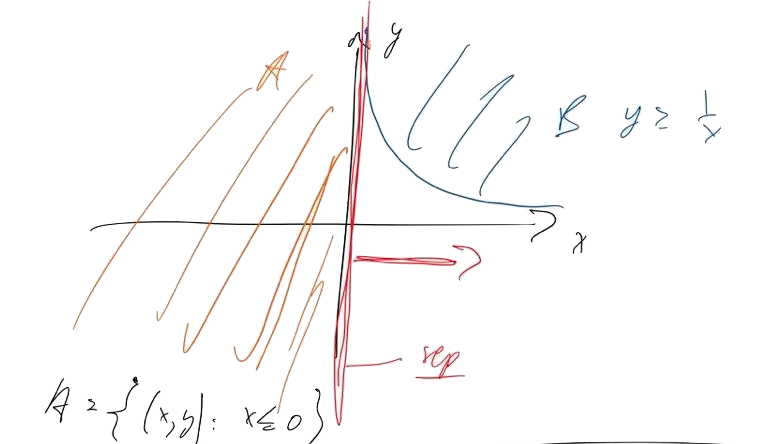
\includegraphics[width=1\textwidth]{fig/lec12-non-strict-separator.png}
  \caption{The sets $A = \{ (x, y): x \leq 0\}$ and $B = \{ (x, y): x
    > 0 \text{ and } y \geq \frac{1}{x} \}$ only permit a non-strictly separating hyperplane.}
  \label{fig:lefthyper}
\end{figure}

One can prove that there exists a non-strictly separating hyperplane for any two disjoint convex sets.
We will prove that if we further require $A$,$B$ to be closed and
bounded, then a strictly separating hyperplane always exists. (Note in
the example above how our choice of $B$ is not bounded.)

\begin{theorem}[Separating Hyperplane Theorem; closed, bounded sets] \label{th:shtcb}
For two closed, bounded, and disjoint convex sets $A, B \in \R^n$ there exists a strictly separating hyperplane $H$.
One such hyperplane is given by normal $\nn = \dd - \cc$ and threshold $\mu = \frac{1}{2}\left(\norm{\dd}_2^2 - \norm{\cc}_2^2\right)$, where $\cc \in A$, $\dd \in B$ are the minimizers of the distance between $A$ and $B$
\begin{equation*} \text{dist}(A, B) = \min_{\aa\in A, \bb \in B}\norm{\aa-\bb}_2 > 0.\end{equation*}
% Note that this distance is strictly larger than zero.
\end{theorem}
\begin{proof}
  We omit the proof that $\text{dist}(A, B) = \min_{\aa\in A, \bb \in
    B}\norm{\aa-\bb}_2 > 0$, which follows from $A,B$ being disjoint,
  closed, and bounded.
Now, we want to show that $\ip{\nn,\bb} > \mu$ for all $\bb \in B$; then $\ip{\nn,\aa} < \mu$ for all $\aa\in A$ follows by symmetry.
Observe that
\vspace{-1em}
\begin{align*}
  \ip{\nn, \dd} - \mu&= \ip{\dd-\cc,\dd} - \frac{1}{2}\left(\norm{\dd}_2^2-\norm{\cc}_2^2\right)\\
                    &= \norm{\dd}_2^2 - \dd^{\trp}\cc - \frac{1}{2}\norm{\dd}_2^2 + \frac{1}{2}\norm{\cc}_2^2 \\
										&= \frac{1}{2}\norm{\dd-\cc}_2^2 > 0.
\end{align*}
So suppose there exists $\uu \in B$ such that $\ip{\nn, \uu} - \mu \leq 0$.
We now look at the line defined by the distance minimizer $\dd$ and the point on the ``wrong side'' $\uu$.
Define $\bb(\lambda) = \dd + \lambda(\uu - \dd)$, and take the derivative of the distance between $\bb(\lambda)$ and $\cc$.
Evaluated at $\lambda=0$ (which is when $\bb(\lambda) = \dd$), this yields
\begin{equation*}
  \left.\frac{d}{d\lambda} \norm{\bb(\lambda) - \cc}_2^2\right\rvert_{\lambda=0} =
	\left.2\ip{\dd-\lambda\dd+\lambda\uu-\cc,\uu-\dd}\right\rvert_{\lambda=0} =
	2\ip{\dd-\cc, \uu-\dd}.
\end{equation*}

However, this would imply that the gradient is strictly negative since
\begin{align*}
\ip{\nn, \uu} - \mu & = \ip{\dd-\cc,\uu} - \ip{\dd-\cc,\dd} + \ip{\dd-\cc,\dd} - \mu \\
                  & = \ip{\dd-\cc,\uu-\dd} + \norm{\dd}_2^2 - \ip{\cc,\dd} - \frac{1}{2}\norm{\dd}_2^2+\frac{1}{2}\norm{\cc}_2^2 \\
                  & = \ip{\dd-\cc,\uu-\dd} + \frac{1}{2}\norm{\dd-\cc}_2^2 \leq 0.
\end{align*}
This contradicts the minimality of $\dd$ and thus concludes this proof.
\end{proof}

A more general separating hyperplane theorem holds even when the sets
are not closed and bounded:

\begin{theorem}[Separating Hyperplane Theorem] \label{th:sht}
Given two disjoint convex sets $A, B \in \R^n$ there exists a hyperplane $H$
separating them.
\end{theorem}


\section{Lagrange Multipliers and Duality of Convex Problems}

In this Section, we'll learn about \emph{Langrange Multipliers} and
how they lead to convex duality.
But first, let's see an example to help illustrate where these ideas
come from.

Imagine you were to prove that for all $\xx \in \R^n$ we have $\norm{\xx}_p \leq n^{\frac{1}{2} - \frac{1}{p}}\norm{\xx}_2$ for some $1 \leq p \leq 2;$.
We can look at this as optimizing $\max_{\xx} \norm{\xx}_p$ subject to $\norm{\xx}_2$ being constant, e.g.\ simply $\norm{\xx}_2 = 1$. Then the statement above follows from a scaling argument.

\begin{figure}[ht]
  \centering
  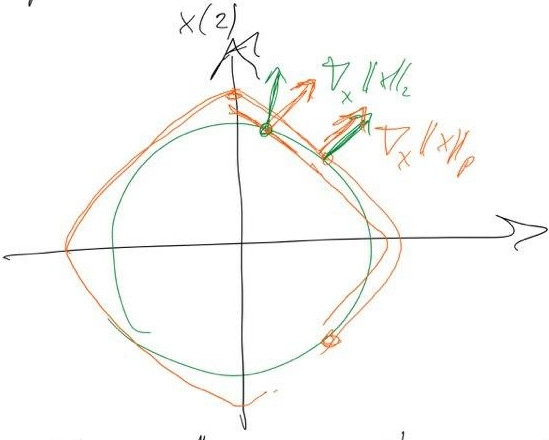
\includegraphics[width=.48\textwidth]{fig/lec12-2p-norms.jpeg}
  \caption{Looking at fixed $\norm{\xx}_p = \alpha$ and $\norm{\xx}_2=1$. (Here, $p = 1.5$.)}
  \label{fig:2-p-norm}
\end{figure}

If we move from $\xx$ to $\xx + \ddelta$ with $\ddelta \perp \grad_{\xx}\norm{\xx}_2$ and $\ddelta \not\perp \grad_{\xx}\norm{\xx}_p$ means that for infinitesimally small $\ddelta$ the 2-norm stays constant but the $p$-norm changes.
That means for either $\xx - \ddelta$ or $\xx + \ddelta$ the $p$-norm
while the 2-norm stays constant. Hence at the maximum of $\norm{\xx}_p$ the gradients of both norms have to be parallel, i.e.~\begin{equation*}\grad_{\xx}\left(\norm{\xx}_p - \lambda\norm{\xx}_2\right) = 0.\end{equation*}
%Here, $\lambda$ is the
This insight is the core idea of Lagrange multipliers (in this case $\lambda$).

Note that here the problem is not convex, because $\{ \xx: \norm{\xx}_2^2 =
1 \}$ is not convex and because we are asking to \emph{maximize} a norm.
In the following we will study Lagrange multipliers for general convex problems.

\subsection{General Convex Problems}

A full formal treament of convex duality would require us to be more careful
about using $\inf$ and $\sup$ in place of $\min$ and $\max$, as well
as considering problems that have no feasible solutions.
Today, we'll ignore these concerns.

Let us consider a general convex optimization problem with convex objective, linear equality constraints and convex inequality constraints
\begin{align}
  \label{eq:primalprob}
     \min_{y \in S}{} & \energy(\yy) \\ \nonumber
\text{s.t.}\  & \AA\yy = \bb \\ \nonumber
              & \cc(\yy) \leq \veczero,
\end{align}
where $\energy(\yy): S \rightarrow \R$ is defined on a convex subset $S \subseteq \R^n$, $\AA \in \R^{m\times n}$
and $\cc(\yy)$ is a vector of constraints $\cc(\yy) = \left(c_i(\yy)\right)_{i \in [k]}$.
For every $i \in [k]$ the function $c_i: S \rightarrow \R$ is convex.

\begin{definition}[Primal feasibility]
We say that $\yy \in S$ is \emph{primal feasible} if all constraints are satisfied, i.e.~$\AA\yy = \bb$ and $\cc(\yy) \leq \veczero$.
\end{definition}

In the following we will denote by $\alpha^* = \energy(\yy^*)$ the optimal value of the primal program where $\yy^*$ is an minimizer.

\begin{definition}
Next we introduce the \emph{dual variables} $\xx \in \R^m$, $\ss \in \R^k$ and define the \emph{Lagrangian} as
\begin{equation*} L(\yy, \xx, \ss) = \energy(\yy) + \xx^{\trp}(\bb-\AA\yy) + \ss^{\trp}\cc(\yy). \end{equation*}
We also define a Lagrangian only in terms of the dual variables by minimizing over $\yy$ as
\begin{equation*} L(\xx, \ss) = \min_{\yy}L(\yy, \xx, \ss). \end{equation*}
\end{definition}

\begin{definition}[Dual feasibility]
We say $(\xx, \ss)$ is dual feasible if $\ss \geq 0$.
If additionally $\yy$ is primal feasible, we say $(\yy, \xx, \ss)$ is primal-dual feasible.
\end{definition}

\begin{definition}[Dual problem]
We define the \emph{dual problem} as
\begin{align}
  \label{eq:dualprob}
  \max_{\substack{\xx, \ss \\ \ss \geq 0}}
  \min_{\yy}L(\yy, \xx, \ss)
  =
  \max_{\substack{\xx, \ss \\ \ss \geq 0}} L(\xx,  \ss)
  \end{align}
and denote the optimal dual value by $\beta^*$.
\end{definition}


For each $\yy$, the Lagrangian $L(\yy, \xx,
\ss)$ is linear in $(\xx,\ss)$ and hence also concave in them.
Hence $L(\xx,  \ss)$ is a concave function, because it is the pointwise
minimum (over $\yy$), of a collection of concave functions in
$(\xx,\ss)$.

This also means that the dual problem is really a convex optimization
problem in disguise, because we can flip the sign of $-L(\xx,  \ss)$
to get a convex function and minimizing this is equivalent to
maximizing $L(\xx,  \ss)$.
\begin{align*}
  \max_{\substack{\xx, \ss \\ \ss \geq 0}} L(\xx,  \ss)
  =
  -
  \min_{\substack{\xx, \ss \\ \ss \geq 0}} -L(\xx,  \ss)
\end{align*}

% Of course, we can write the dual problem using the
% $\min_{\yy}L(\yy, \xx, \ss)$ notation as
% \[
%   \max_{\substack{\xx, \ss \\ \ss \geq 0}}
%   \min_{\yy}L(\yy, \xx, \ss)
%   =
%   \max_{\substack{\xx, \ss \\ \ss \geq 0}} L(\xx,  \ss)
%   \]



\subsection{Weak Duality}
\label{sec:weakdual}
First we see that the primal problem can be written in terms of the Lagrangian as
\begin{equation}
  \label{eq:primalminmax}
  \alpha^* = \min_{\yy}\max_{\xx; \ss\geq\veczero} L(\yy, \xx, \ss)
\end{equation}
This is because for a minimizing $\yy$ all constraints have to be satisfied and the Lagrangian simplifies to $L(\yy,\xx,\ss) = \energy(\yy)$.
If $\AA\xx - \bb = \veczero$ was violated, making $\xx$ large sends $L(\yy,\xx,\ss) \rightarrow \infty$.
And if $\cc(\yy) \leq \veczero$ is violated, we can make $L(\yy,\xx,\ss) \rightarrow \infty$ by choosing large $\ss$.

Note that we require $\ss \geq \veczero$, as we only want to penalize the violation of the inequality constraints in one direction, i.e.\ when $\cc(\yy) > 0$.

%\begin{theorem}[Weak Duality]
For any primal-dual feasible $\yy,\xx,\ss$ we have
$L(\yy, \xx, \ss) \leq \energy(\yy)$ and hence also $L(\xx, \ss) = \min_y L(\yy, \xx, \ss) \leq \energy(\yy)$.

In other words $\max_{\xx; \ss \geq 0} L(\xx, \ss) = \beta^* \leq \alpha^*$.
This is referred to as \emph{weak duality}.

Using the forms in Equations~\eqref{eq:dualprob} and
\eqref{eq:primalminmax}, we can also state this as
\begin{equation*}
  \alpha^* = \min_{\yy}\max_{\xx; \ss\geq\veczero} L(\yy, \xx, \ss)
  \geq
  \max_{\xx; \ss\geq\veczero} \min_{\yy} L(\yy, \xx, \ss)
  =
  \beta^*
  .
\end{equation*}

\subsection{Strong Duality}
So now that we have proved weak duality $\beta^* \leq \alpha^*$,
what is strong duality? $\beta^* = \alpha^*$?
The answer is yes, but strong duality only holds under some conditions.

One sufficient condition we look at today is a variant of \emph{Slater's condition}%

\begin{definition}[Slater's condition with full domain] \label{def:slater}
A (primal) problem as defined in \eqref{eq:primalprob} with $S = \R^n$ fulfills
Slater's condition if there exists a \emph{strictly feasible} point,
i.e.\ there exists $\yytil$ s.t.\ $\AA\yytil = \bb$ and $\cc(\yytil) <
\veczero$.
This means that the strictly feasible point $\yytil$ lies strictly inside the set $\{\yy : \cc(\yy) \leq \veczero\}$ defined by the inequality constraints.
\end{definition}

\begin{theorem}
  \label{thm:slaterstrongduality}
For a problem satisfying Slater's condition, strong duality holds, i.e.\ $\alpha^* = \beta^*$.
In other words, the optimal value of the primal problem $\alpha^*$ is equal to the optimal value of the dual.
\end{theorem}

To extend Slater's condition to the case when the domain $S$ is a
strict subset of $\R^n$, we need the notion of a ``relative interior''.

% \begin{definition}[Affine hull] \label{def:affhull}
% Given a set $S \subset \R^n$, the \emph{affine hull} of $S$, denoted $\operatorname{aff}(S)$, is the
% union of $S$ and all lines through any pair of points in $S$.
% We can also write this as
% \[
%   \operatorname{aff}(S) = \setof{\alpha \xx + (1-\alpha) \yy : \xx,
%     \yy \in S, \alpha \in \R}. 
%   \]
% \end{definition}

\begin{definition}[Relative interior] \label{def:relint}
  Given a convex set $S \subset \R^n$, the \emph{relative interior} of $S$ is
  \[
    \operatorname{relint}(S) = \setof{x \in S : \text{ for all } \yy
      \in S \text{ there exists } \epsilon > 0 \text{ such that }
      \xx - \epsilon(\yy - \xx) \in S}
    .
  \]
\end{definition}
In other words, $\xx \in \operatorname{relint}(S)$ if starting at $\xx
\in S$ we can move
``away'' from any $\yy \in S$ by a little and still be in $\SS$.
As an example, suppose $S = \setof{(s,t) \in \R^2 \text{ such that } s
  \geq 0 \text{ and } t = 0}$.
Then $(0,0) \in S$ but $(0,0) \not\in \operatorname{relint}(S)$, while
$(1,0) \in \operatorname{relint}(S)$.

Now, we can state a more general version of Slater's condition.

\begin{definition}[Slater's condition] \label{def:slatergeneral}
A (primal) problem as defined in \eqref{eq:primalprob} fulfills
Slater's condition if there exists a \emph{strictly feasible} point
$\yy \in \relint(S)$.
We require $\AA\yytil = \bb$ and $\cc(\yytil) <
\veczero$.
This means that the strictly feasible point $\yytil$ lies strictly inside the set $\{\yy : \cc(\yy) \leq \veczero\}$ defined by the inequality constraints.
\end{definition}

Theorem~\ref{thm:slaterstrongduality} also holds given the general
Slater's condition of Definition~\ref{def:slatergeneral}.

\paragraph{How are we going to prove this?} Before we prove the theorem, let's make a few observations to get us
warmed up. If you get bored, skip ahead to the proof.

It is sufficient to prove that $\alpha^* \leq \beta^*$, as the statement then follows in conjunction with weak duality.
We define the set
\begin{equation*} G = \{(\energy(\yy), \AA\yy - \bb, \cc(\yy)) : \yy \in S \}, \end{equation*}
where $S \subseteq \R^n$ is the domain of $\energy$.

Immediately, we observe that we can write the optimal primal value as
\begin{equation*} \alpha^* = \min \{t:(t,\vv,\uu) \in G, \vv = \veczero, \uu \leq \veczero\}. \end{equation*}
Similarly, we can write the Lagrangian (after minimizing over $\yy$)
\begin{equation*} L(\xx, \ss) = \min_{(t,\vv,\uu) \in G} (1, \xx, \ss)^{\trp} (t, \vv, \uu). \end{equation*}
This is equivalent to the inequality, for $(t,\vv,\uu) \in G$,
\begin{equation*} (1, \xx, \ss)^{\trp}(t, \vv, \uu) \geq L(\xx, \ss). \end{equation*}
which defines a hyperplane with $\nn = (1,\xx,\ss)$ and $\mu = L(\xx,
\ss)$ such that $G$ is on one side.

To establish strong duality, we would like to show the existence of a
hyperplane such that for $(t,\vv,\uu) \in G$
\[
  \nn^{\trp}(t, \vv, \uu) \geq \alpha^* \text{ and } \nn = (1,\xxhat,\sshat)
  \text{ with } \sshat \geq \veczero.
\]
Then we would immediately get
\begin{equation*}
 \beta^* \geq L(\xxhat,\sshat)= \min_{(t,\vv,\uu) \in G} (1, \xx,
 \ss)^{\trp} (t, \vv, \uu) \geq \alpha^* .
\end{equation*}

Perhaps not surprisingly, we will use the Separating
Hyperplane Theorem.
What are the challenges we need to deal with?
\begin{itemize}
\item We need to replace $G$ with a convex set (which we will call
  $A$) and separate $A$ from some other convex set (which we will call $B$).
\item We need to make sure the hyperplane normal $\nn$ has $1$ in the first
  coordinate and $\ss \geq \veczero$, and the hyperplane threshold is $\alpha^*$.
\end{itemize}

% The proof we are about to see handles these things in one neat
% stroke: Essentially, we replace $G$ with the convex set that comes from replacing
% the convex functions $\energy$ and $\cc$ with their epigraphs.

% If strong duality indeed holds,
% and is obtained at some $L(\yyhat,\xxhat,\sshat)$
% then the reasoning we used to prove weak duality in
% Section~\ref{sec:weakdual} seems to suggest that a dual point
% $(\xx^*,\ss^*)$ maximizing $L(\xx,\ss)$ will occur at a feasible
% $\yy$, since otherwise $L(\yy,\xx,\ss)$ could be reduced further by
% changing $(\xx,\ss)$ to penalize $\yy$.
% Of course, it's not clear whether this could then be counter-acted by
% changing $\yy$.


% \begin{itemize}
% \item and correspond to a feasible $\yy$ in the sense that
%   $L(\xx^*,\ss^*) = (\yy,\xx^*,\ss^*)$
%   \item be dual feasible,
% \end{itemize}
% If the minimizing $\yy$ is not feasible,  but



%  Then by considering a feasible $\yyhat$ for the primal problem, we
%   get
%   \begin{align**}
%     \beta^*
%     & \geq L(\xxhat,\sshat) \\
%     &= (1, \xxhat,\sshat)^{\trp}(\energy(\yyhat), \AA\yyhat - \bb, \cc(\yyhat))
%       \geq \energy(\yyhat) \geq \alpha^*
%   \end{align**}
% This sandwiching also tells us that $\yyhat$ and $(\xxhat,\sshat)$
% must be optimal for the primal and dual problems respectively.

% Clearly, we like to ensure that


% We'd like to show that
% for some dual-feasible $(\xxhat,\sshat)$ maximizing $L(\xx,
% \ss)$, then the hyperplane inequality doesn't have any slack, i.e. it
% holds with equality at some point, and furthermore, equality is
% obtained at some $(t, \vv, \xx) = (\energy(\yyhat), \AA \yyhat - \bb,
% \cc(\yyhat))$ where $\yyhat$ is feasible.





% When we proved weak duality in Section~\ref{sec:weakdual}, our reasoning

\begin{proof}[Proof of Theorem~\ref{thm:slaterstrongduality}.]
  For simplicity, our proof will assume that $S = \R^n$, but only a little
  extra work is required to handle the general case.

  Let's move to on finding two convex disjoints sets $A, B$ to enable the use of the separating hyperplane \autoref{th:sht}.

First set we define $A$, roughly speaking, as a multi-dimensional epigraph of
$G$. More precisely
\begin{equation*} A = \{(t, \vv, \uu) : \exists \yy \in S, t \geq \energy(\yy), \vv = \AA\yy - \bb, \uu \geq \cc(\yy)\}. \end{equation*}
Note that $A$ is a convex set. The proof is similar to the proof that the epigraph of a convex function is a convex set.
The optimal value of the primal program can be now written as
\begin{equation*} \alpha^* = \min_{(t,\veczero,\veczero) \in A} t. \end{equation*}
And we define another set $B$ of the same dimensionality as $A$ by
\begin{equation*} B := \{(r \in \R, \veczero \in \R^m, \veczero \in \R^k) : r < \alpha^* \}. \end{equation*}
This set $B$ is convex, as it is a ray.
An example of two such sets $A,B$ is illustrated in \autoref{fig:ab}.

We show that $A \cap B = \emptyset$ by contradiction.
Suppose $A, B$ are not disjoint; then there exists $\yy$ such that
\begin{equation*} (\energy(\yy), \AA\yy-\bb, \cc(\yy)) = (r, \veczero, \uu) \end{equation*}
with $\uu \leq \veczero$.
But this means that $\yy$ is feasible and  $\energy(\yy) = r < \alpha^*$; contradicting the optimality of $\alpha^*$.

% Now let's move back to proving that strong duality follows from Slater's condition.
%As Slater's condition requires the existence of a $\yy$ such that $\AA\yy = \bb$
To make things simpler,
we assume that our linear constraint matrix $\AA \in \R^{m\times n}$,
has full row rank and $m < n$ (but very little extra work is required to
deal with the remaining cases, which we omit).

As we just proved, $A$ and $B$ are convex and disjoint sets and hence the separating hyperplane theorem (\autoref{th:sht}) we introduced earlier in this chapter implies the existence a separating hyperplane.
This means there exists a normal
$\nn = (\tilde\rho, \xxtil, \sstil)$ and threshold
% \footnote{To prevent confusion, the threshold here is denoted $\mu$ instead of $alpha$} %
$\mu$ and with $A$ on one side, i.e.\
%\begin{equation*} (t, \vv, \uu) \in A \implies \begin{pmatrix}t \vv^{\trp} \uu^{\trp}\end{pmatrix}\begin{pmatrix}\tilde\rho \\ \xxtil \\ \sstil\end{pmatrix} \geq \alpha \end{equation*}
\begin{equation} \label{eq:A}
(t, \vv, \uu) \in A \implies (t, \vv, \uu)^{\trp}(\tilde\rho, \xxtil, \sstil) \geq \mu
\end{equation}
and the set $B$ on the other side:
\begin{equation} \label{eq:B}
(t, \vv, \uu) \in B \implies (t, \vv, \uu)^{\trp}(\tilde\rho, \xxtil, \sstil) \leq \mu.
\end{equation}

Now, we claim that $\sstil \geq 0$. Suppose $\sstil(i) < 0$, then for $\uu(i) \rightarrow \infty$ the threshold would grow unbounded, i.e.\ $\mu \rightarrow -\infty$ contradicting that the threshold $\mu$ is finite by the separating hyperplane theorem.
Similarly we claim $\tilde\rho \geq 0$, as if this were not the case, having $t \rightarrow \infty$ implies that $\mu \rightarrow -\infty$ again contradicting the finiteness of $\mu$.

From Equation~\eqref{eq:B} it follows that $t\tilde\rho \leq \mu$ for all $t < \alpha^*$ which implies that $t\tilde\rho \leq \mu$ for $t = \alpha^*$ by taking the limit. Hence we have $\alpha^*\tilde\rho \leq \mu$.
From $(t, \vv, \uu) \in A$ we get from  Equation~\eqref{eq:A}
\begin{equation*}
(\tilde\rho, \xxtil, \sstil)^{\trp}(t, \vv, \uu) \geq \mu \geq \alpha^*\tilde\rho
\end{equation*}
and thus
\begin{equation}\label{eq:rhotilde}
(\tilde\rho, \xxtil, \sstil)^{\trp}(\energy(\yy), \AA\yy-\bb,\cc(\yy)) \geq \alpha^*\tilde\rho.
\end{equation}


Now we consider two cases; starting with the ``good'' case where $\tilde\rho > 0$.
Dividing  Equation~\eqref{eq:rhotilde} by $\tilde\rho$ gives
\begin{equation*}
  \energy(\yy) + \frac{\xxtil^{\trp}}{\tilde\rho}(\AA\yy - \bb) + \frac{\sstil^{\trp}}{\tilde\rho}\cc(\yy) \geq \alpha^*.
\end{equation*}
Noting that the left hand side above is $L(\yy, \frac{\xxtil}{\tilde\rho}, \frac{\sstil}{\tilde\rho})$
and that the equation holds for arbitrary $\yy$; therefore also for the minimum we get
\begin{equation*} \min_{\yy}{L\left(\yy, \frac{\xxtil}{\tilde\rho}, \frac{\sstil}{\tilde\rho}\right)}\geq \alpha^* \end{equation*}
and hence via definition of $\beta^*$ finally
\begin{equation*} \beta^* \geq L\left(\frac{\xxtil}{\tilde\rho},\frac{\sstil}{\tilde\rho}\right) \geq \alpha^*. \end{equation*}

Next consider the ``bad'' case $\tilde\rho = 0$.
As $\alpha^*\tilde\rho \leq \mu$, we have $0 \leq \mu$.
From  Equation~\eqref{eq:A} we get
\begin{equation*}
  \cc(\yy)^{\trp}\ss + \xx^{\trp}(\bb-\AA\yy) \geq \mu \geq 0.
\end{equation*}
As Slater's condition holds, there is an interior point $\yytil$, i.e.\ it satisfies $\bb - \AA\yytil = \veczero$ and $\cc(\yytil) < \veczero$. Together with the equation above this yields
\begin{equation*} \cc(\yytil)^{\trp}\sstil + \xxtil^{\trp}\veczero \geq 0 \end{equation*}
which implies
$\cc(\yytil)^{\trp}\sstil \geq 0 $
and as $\cc(\yytil) < \veczero$ this means $\sstil = \veczero$.

As the normal $(\tilde\rho,\sstil,\xxtil)$ of the hyperplane can not be all zeroes, this means the last ``component'' $\xxtil$ must contain a non-zero entry, i.e.\ $\xxtil \neq \veczero$.
Furthermore $\xxtil^{\trp}(\bb - \AA\yytil) = \veczero$, $\cc(\yytil) < \veczero$ and $\AA$ has full row rank, hence there exists $\ddelta$ such that
\begin{equation*}
\xxtil^{\trp}(\bb-\AA(\yytil+\ddelta)) < \veczero \text{ and } \cc(\yytil + \ddelta) < 0.
\end{equation*}
This, however, means that there is a point in $A$ on the wrong side of the hyperplane, as
\begin{equation*}
(\tilde\rho, \xxtil, \sstil)^{\trp}(\energy(\yytil+\ddelta), \bb-\AA(\yytil+\ddelta), \cc(\yytil+\ddelta)) < 0
\end{equation*}
but the threshold is $\mu \geq 0$.
\end{proof}

\begin{remark*}
  Note that our reasoning about why $\ss \geq \veczero$ in the proof
  above is very similar to our reasoning for why the primal program
  can be written as Problem~\eqref{eq:primalminmax}.
\end{remark*}

\paragraph{Example.}
As an example of $A$ and $B$ as they appear in the above proof,
consider
\[
\min_{\substack{y \in (0,\infty) \\ 1/y
    -1 \leq 0}}
y^2
\]
 This leads to $\alpha^* = 1,
    y^* =1$, and $A = \setof{ (t,u): y \in (0,\infty) \text{ and } t >y^2
       \text{ and } u \geq 1/y-1}$, and $B = \setof{ (t,0) : t < 1}$ and the separating hyperplane normal is $\nn = (1,2)$.
These two sets $A,B$ are illustrated in \autoref{fig:ab}.
\begin{figure}[H]
  \centering
  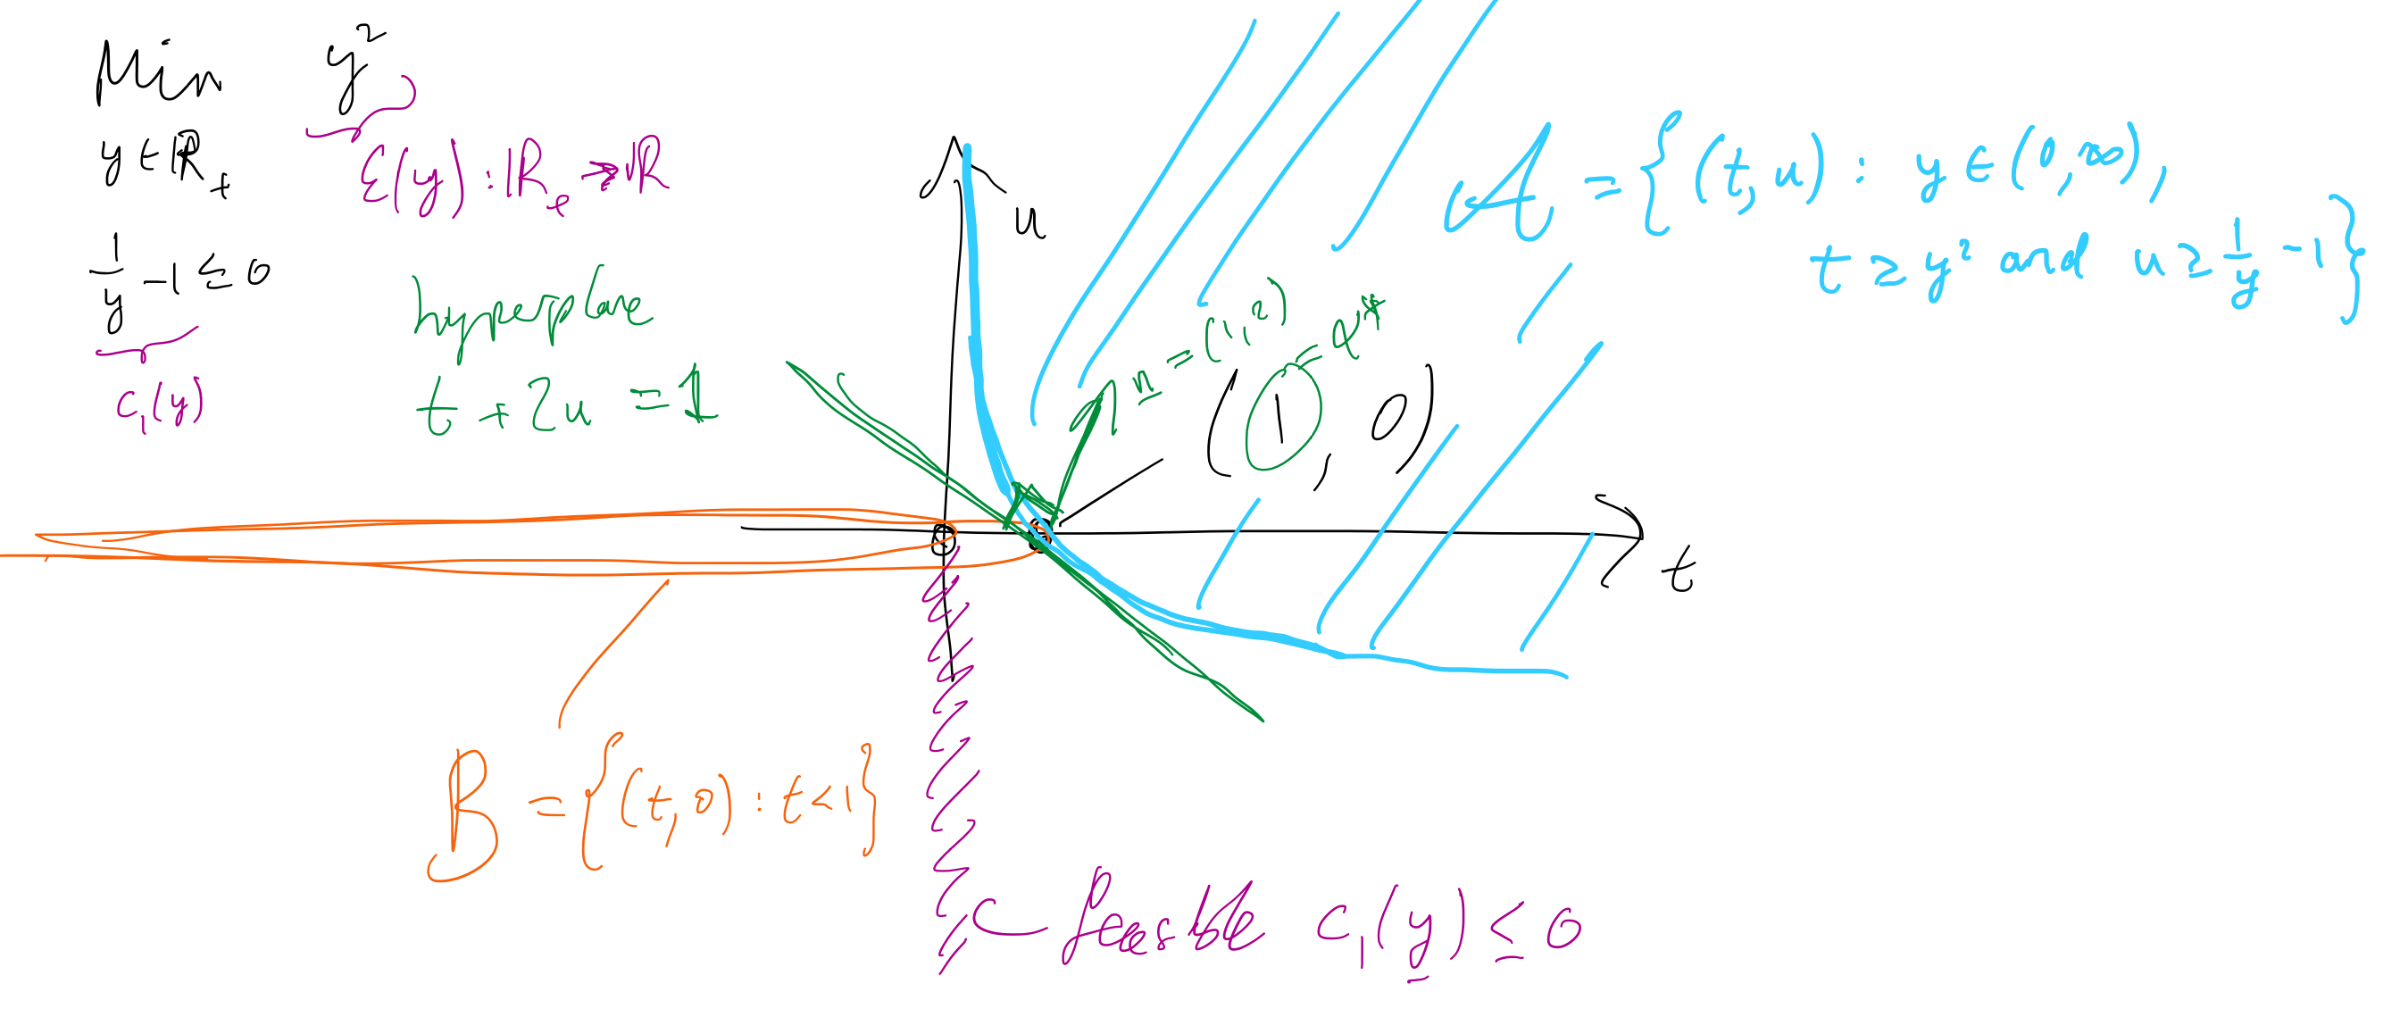
\includegraphics[width=.9\textwidth]{fig/lec12-the-sets-a-b.jpg}
  \caption{Example of the convex sets $A$ and $B$ we wish to separate by hyperplane.}
\label{fig:ab}
\end{figure}



\subsection{The Gradient Perspective}
Let's come back to what we said earlier about parallel gradient.
Suppose $\yy^*$ is an optimizer of the primal problem and $\xx^*, \ss^*$ for the dual.
We thus have
\[ L(\yy^*, \xx^*, \ss^*) = \alpha^* = \beta^*. \]
Because $L(\yy, \xx^*, \ss^*)$ is a convex function in $\yy$, it also
follows that if $\energy: S \to \R$ and $\cc$ are differentiable and the minimizer
$\yy^*$ is not on the boundary of $S$, then we must have that the
gradient w.r.t. $\yy$ is zero, i.e.
\begin{equation*} \left.\grad_{\yy}L(\yy, \xx^*, \ss^*)\right|_{\yy=\yy^*} = 0 \end{equation*}
and plugging in
\[ L(\yy, \xx^*, \ss^*) = \energy(\yy) + \xx^{\trp}(\bb - \AA\yy) + \ss^{\trp}\cc(\yy) \]
yields
\begin{equation*} \grad\energy(\yy) + \xx^{\trp}\grad_y(\bb-\AA\yy) + \ss^{\trp}\grad\cc(\yy) = \veczero. \end{equation*}
And this connects to our point of the parallel gradients from the beginning of this section.

\subsection{Complementary Slackness}

We will see more of this next time, but if we look at $\yy^*$ we see that
\begin{equation*}\energy(\yy^*) =  \alpha^* = \energy(\yy^*) + \xx^{\trp}(\bb - \AA\yy^*) + \ss^{\trp}\cc(\yy^*) = \energy(\yy^*) + \ss^{\trp}\cc(\yy^*) \end{equation*}
and hence when the $i$-th convex constraint is not active, i.e.\ $c_i(\yy^*) < 0$ the \emph{slack} must be zero, i.e.\ $\ss(i) = 0$.
Conversely if the slack is non-zero, that is $\ss(i) \neq 0$ implies that the constraint is active, i.e.\ $c_i(\yy^*) = 0$.

A good reference for this is Boyd's free online book ``Convex
optimization'' (linked to on the course website).
It provides a number of different interpretations of duality. One
particularly interesting one comes from economics:
economists see the slack variables $\ss$ as prices for violating the constraints.

%\end{document}
%%% Local Variables:
%%% mode: latex
%%% TeX-master: "agao21_script"
%%% End:
